\section{Node Collapse}
In a parallel DAG task, one approach to introduce inter-thread cache benefit is to execute nodes with the same code segment/executable object on the same core. This approach allows the second node to re-use cache blocks loaded into the cache by the first node, and reduce the total time required to load instructions into the cache (or memory demand). To obtain inter-thread cache benefit, this paper focusses on the approach of executing nodes with same code segment on the same core. 

This section introduces the collapse of two nodes in a DAG to enable execution of two nodes on the same core. Two nodes $u, v$ of the DAG $G_i$ that have the same code segment can be collapsed into one node $\hat{u} \in \hat{G_i}$. The collapsed node, $\hat{u}$, represents the execution of threads from $u$ and $v$ and maintains parent and child dependencies of $u$ and $v$. Assuming that, for two nodes $x, v \in V_i$, $x \prec^{1} v$ denotes that $x$ is the parent of node $v$ in the DAG $G_i$, then collapse of two nodes is defined as follows:
 \begin{definition}[\textbf{Collapse}]
When two nodes $u,v \in V_i$ of a DAG $G_i$ are collapsed into $\hat{u} \in \hat{V_i}$, the collapsed node $\hat{u}$ must adhere to the following properties:
\begin{itemize}
\item The collapsed node $\hat{u}$ is represents the thread executions of node $u$ and node $v$ and is expressed as $\hat{u} = \langle \alpha_u , c_u(\eta_{\hat{u}}), \eta_{\hat{u}} = \eta_u+\eta_v \rangle$.
\item All parent dependencies of $v$ are maintained by $\hat{u}$, i.e., $ x \prec^{1} \hat{u} \text{ in } \hat{G_i} \, \forall x \prec^1 v \text{ in } G_i$.
\item All child dependencies of $v$ are maintained by $\hat{u}$, i.e., $\hat{u} \prec^{1} y \text{ in } \hat{G_i} \, \forall v \prec^1 y \text{ in } G_i$.
\item All parent dependencies of $u$ are maintained by $\hat{u}$, i.e., $ x \prec^{1} \hat{u} \text{ in } \hat{G_i} \, \forall x \prec^1 u \text{ in } G_i$.
\item All child dependencies of $u$ are maintained by $\hat{u}$, i.e., $\hat{u} \prec^{1} y \text{ in } \hat{G_i} \, \forall u \prec^1 y \text{ in } G_i$.
\end{itemize}
 \end{definition}

During the execution of task $\tau_i$, the greedy scheduler that schedules each node on the dedicated $m_i$ cores treats the collapsed node as a single node executing multiple threads. Thus, collapsing two nodes ensures that they execute on the same core and reduce the memory demand. 

Collapsing two nodes $u, v$ into $\hat{u}$ is the same as collapsing them into $\hat{v}$ since the collapsed node $\hat{u}$ or $\hat{v}$ includes dependencies of both $u$ and $v$. For the sake of simplicity in explanation, if one node $u \in V_i$ is on the critical path of $G_i$, then $v$ is collapsed into $u$ and is referred as $\hat{u}$.





\begin{figure}
  \centering
  \begin{subfigure}[b]{0.4\textwidth}{
      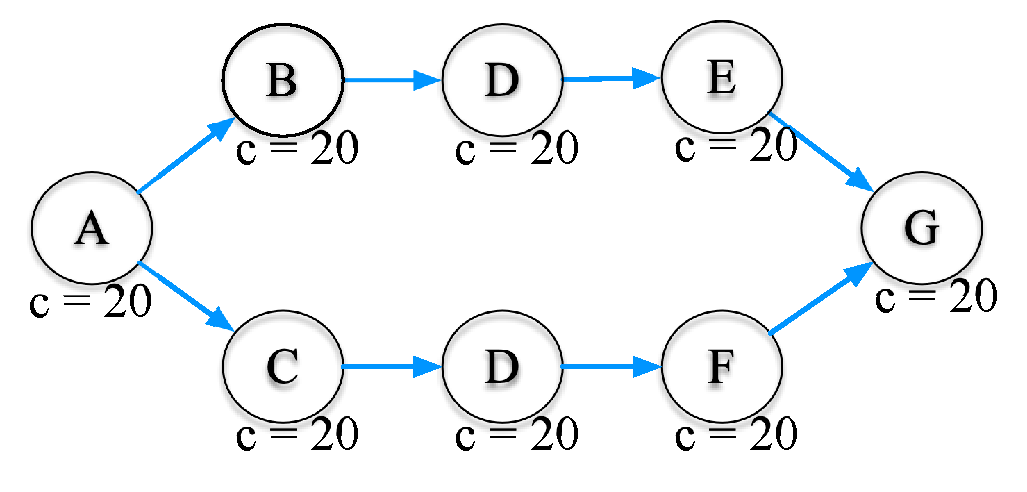
\includegraphics[width=\textwidth]{beforeCollapse}
      \caption{Before Collapse}
      \label{fig:before-collapse}
    }
  \end{subfigure} \quad
  \begin{subfigure}[b]{0.4\textwidth}{
      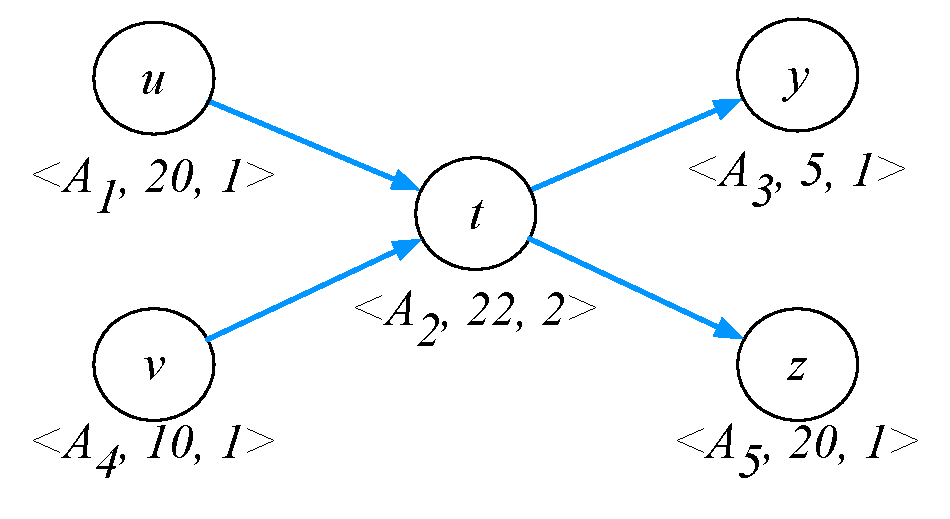
\includegraphics[width=\textwidth]{afterCollapse}
      \caption{After Collapse}
      \label{fig:after-collapse}
    }
  \end{subfigure}
  \caption{An example showing collapse of two nodes}
  \label{fig:dag-collapse}
\end{figure}

Fig.~\ref{fig:dag-collapse} illustrates the collapse of two nodes. Nodes in
Fig.~\ref{fig:before-collapse} are labeled with their node ID and show the tuple representation, i.e., code segment, worst-case execution time and the number of threads executing the node. In Fig.~\ref{fig:before-collapse}, nodes $w$ and $x$ execute one thread each over the same code segment $A_2$ with worst-case execution time of 20 time units. These two nodes can be collapsed into a single node $\hat{w}$ with two threads of execution over code segment $A_2$,  as shown in Fig.~\ref{fig:after-collapse}. Assuming that $A_2$ can fit into the cache and the ratio of memory demand to execution demand is $10:1$, the worst-case execution time of $\hat{w}$ only includes the memory demand of one thread and execution demand of two threads, i.e., $24$ time units.

%% \revise{A property of collapse must be stated. When collapsing two
%%   nodes ${u,v \in V}$ to one node ${u}$ the length of the critical
%%   path is reduced by the WCET of ${v}$ before collapse and increased
%%   by the WCET of ${u}$ after collapse}  





\section{Candidacy for collapse}
\label{sec:candidacy}
Although the previous section mentions that a collapse of nodes can reduce the memory demand of a node,  in some cases, the collapse of two nodes can render the task not schedulable. In this paper, a pair of nodes are said to be candidates for collapse if they can potentially reduce the memory demand of the nodes. This section presents the conditions for a pair of nodes to be called a candidate. For a task ${\tau_i \in \tau}$, associated DAG ${G_i \in \mathbb{G}}$,
where ${G_i = (V, E)}$, the nodes ${u,v \in V}$ qualify as
\emph{candidates} for collapse if and only if the following conditions
are true: 
\begin{enumerate}
  \item Nodes ${u}$ and ${v}$ refer to execution of the same object.
  \item Collapsing ${u}$ and ${v}$ cannot not introduce a cycle in the collapsed DAG $\hat{G_i}$.
  %% I believe this condition is covered in the cbound. We can discuss this on saturday.
  \item \revise{The sum of the individual worst-case execution times of ${u}$
    and ${v}$ is greater than the collapsed worst-case execution time
    of ${u}$ and ${v}$ i.e. ${c(\eta_u) + c(\eta_v) > c(\eta_u + \eta_v)}$.}
\end{enumerate}

The first property of candidacy is that the candidate nodes $u$ and $v$ should represent the execution over the same code segment. The collapse of two nodes with different code segments can introduce context switch delays and cache evictions, which does not provide any inter-thread cache benefit. On the contrary, it can increase the worst-case execution time. 


%%Another property of candidacy is that execution of two thread on the same core should be less sequential execution of both the blocks, i.e., ${c(\eta_u) + c(\eta_v) > c(\eta_u + \eta_v)}$. 

\begin{figure}
  \centering
  \begin{subfigure}[b]{0.48\textwidth}{
      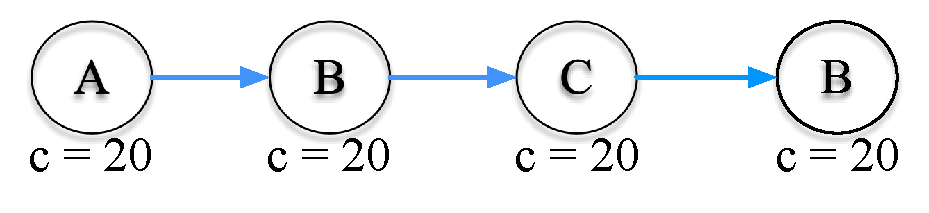
\includegraphics[width=\textwidth]{beforeViolation}
      \caption{Before Collapse}
      \label{fig:beforeViolation}
    }
  \end{subfigure}~
  \begin{subfigure}[b]{0.33\textwidth}{
      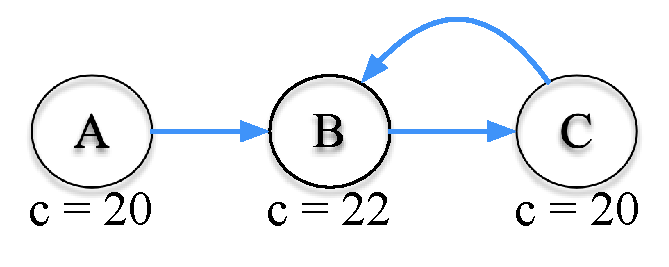
\includegraphics[width=\textwidth]{afterViolation}
      \caption{After Collapse}
      \label{fig:afterViolation}
    }
  \end{subfigure}
  \caption{Collapse of two nodes can result in a loop inside the DAG task}
  \label{fig:dag-violation}
\end{figure}


The second property of candidacy is that the collapse of two nodes should not introduce any loops in the collapsed DAG.  If a loop exists in the collapsed DAG, the first node in the cycle $\hat{u}$ is a predecessor of itself, i.e., $\hat{u} \prec^{*} \hat{u}$. This implies that the first node does not meet its dependency and is never released. Thus, the task is no longer schedulable. For example, in Fig.~\ref{fig:dag-violation}, node $\hat{v}$ is never release as it is waiting for $w$, and $w$ is never release as it is waiting for node $\hat{v}$. Considering \textbf{${d(u, v)}$} defines the greatest number of edges along a directed path from $u$ to $v$ (and ${d(u,v) = 0}$ when no path exists), the necessary and sufficient condition for a pair of nodes to not introduce a loop when collapsed is as follows:

%% removed after revised text
%%\textbf{Definition ${d(u, v)}$} -- is the greatest number of edges
%%along a directed path from ${u}$ to ${v}$ in ${G}$. When no path
%%exists, ${d(u,v) = 0}$.

\begin{theorem}[\textbf{Collapse does not introduce a loop}]
  For a DAG ${G = (V, E)}$ and nodes ${u, v \in V}$ where ${u \prec^{*}
    v}$, ${u}$ and ${v}$ can be collapsed without introducing a loop
  if and  only if ${d(u, v) \le 1}$.
\end{theorem}
\begin{proof}
This proof is divided into two parts. The first part proves the necessary condition, i.e., if the constraint is violated, then the collapse of two nodes will introduce a loop. The second part proves the sufficient condition, i.e., a loop is introduced in a DAG after collapse only if the constraint is violated. 

For the first part, $d(u, v) > 1$ implies that there exists a node $t$ such that $t$ is a predecessor of $v$ ($t \prec^{*} v$) and $u$ is a predecessor of $t$ ($u \prec^{*} t$). When nodes $u$ and $v$ are collapsed into $\hat{v}$, by the definition of collapse, $t$ is predecessor of $\hat{v}$ and $\hat{v}$ is a predecessor of $t$. Thus, the violation of the constraint introduces a loop. 

For the second part, a DAG violation in the collapsed DAG $\hat{G_i}$ implies that there exists a path from $w$ to $w$ with length greater than $1$, i.e., $w \prec{x} w$ and $x > 1$.  Since there are no loops in the original DAG $G_i$, only a collapsed node $\hat{u}$ can cause a loop in the collapsed DAG, i.e. $w = \hat{u}$. This implies that, if there exists a node $t \in \hat{G_i}$ such that $t \prec^{*} w$ and $w \prec^{*} t$ then in the original DAG $G_i$ these dependencies correspond to $t \prec^{*} v$ and $u \prec^{*} t$. If there exists a $t$ such that $u \prec^{*} t \prec^{*}$, then the length of path from $u$ to $v$ is at least $2$. Thus, a loop is introduced in the collapsed DAG violation only when $d(u, v) > 1$. 

Therefore, we can conclude that two nodes $u$ and $v$ in a DAG task $\tau_i$ when collapsed do not introduce a loop if and only if $d(u, v) \le 1$.
\end{proof}

In summary, we define the candidates for collapse as follows:
\begin{definition}[\textbf{Candidates for Collapse}]
Two nodes $u, v \in V_i$, where ${u \prec^{*} v}$, are defined as {\textbf candidates for collapse} if they conform to the following properties:
\begin{itemize}
 \item Nodes ${u}$ and ${v}$ refer to execution of the same object.
  \item $d(u, v) \le 1$
  %% I believe this condition is covered in the cbound. We can discuss this on saturday.
  \item \revise{The sum of the individual worst-case execution times of ${u}$
    and ${v}$ is greater than the collapsed worst-case execution time
    of ${u}$ and ${v}$ i.e. ${c(\eta_u) + c(\eta_v) > c(\eta_u + \eta_v)}$.}
\end{itemize}
\end{definition}
